\subsection{Метод локальных массовых соотношений LMR2021}
В отличие от рассмотренных выше ядерных моделей, подход локальных массовых соотношений не описывает структуру и физику ядра, а использует закономерности, связывающие массы соседних изотопов. Обычно это дифференциальные выражения, которые можно применять рекурсивно, начиная с ядер, энергии связи которых известны из эксперимента, и уходя сколь угодно далеко в область экзотических изотопов. Таким образом, имея набор экспериментальных данных, можно шаг за шагом получать массы нуклидов вплоть до границ области существования ядер.

Метод локальных массовых соотношений предложен в~\cite{garvey1966} и актуален до сих пор благодаря высокой точности (отмеченной, например, в~\cite{bao2014}) при сравнительной простоте вычислений. Еще одним достоинством подхода является разнообразие вариантов самого массового соотношения: можно подобрать такое выражение, которое будет наиболее удобно в конкретном исследовании.

\subsubsection{Остаточное протон-нейтронное взаимодействие}
В настоящей работе наряду с таблицами FRDM2012 и HFB-24 используется таблица теоретических ядерных масс LMR2021~\cite{vladimirova2022}, рассчитанная при помощи соотношения, которое связывает массы четырех соседних изотопов, расположенных на $NZ$-диаграмме в виде квадрата два на два, через энергию остаточного протон-нейтронного взаимодействия $\Delta_{np}$. Эта величина введена в работе~\cite{kravtsov1959} и впервые использовалась для оценки энергий связи ядер в~\cite{janecke1974}. Для ядра, состоящего из $Z$ протонов и $N$ нейтронов, величина $\Delta_{np}$ выражается как
\begin{equation}\label{eq:np-interaction}
  \begin{aligned}
    \Delta_{np}(N,Z) &= S_{np}(N,Z) - [S_{p}(N-1,Z) + S_{n}(N,Z-1)] = \\
    &= B(N,Z) + B(N-1,Z-1) - B(N,Z-1) - B(N-1,Z),
  \end{aligned}
\end{equation}
где $S_n$, $S_p$, $S_{np}$ --- энергии отделения нуклонов и их пары, а $B(N,Z)$ --- энергия связи ядра с $N$ нейтронов и $Z$ протонов.

Таким образом масса любого ядра может быть вычислена, если известны энергии связи трех соседних изотопов, образующих вместе с рассматриваемым ядром квадрат на $NZ$-диаграмме, а также соответствующее значение энергии $\Delta_{np}$. В ряде случаев для одного ядра можно построить несколько таких квадратов, тогда в качестве оценки неизвестной энергии связи имеет смысл брать средний результат.

\subsubsection{Аппроксимация энергии протон-нейтронного взаимодействия}
На рис.~\ref{fig:delta_np} показана экспериментальная зависимость энергии протон-нейтронного взаимодействия от массового числа. Как видно, для ядер с четными и нечетными массовыми числами по отдельности величина $\Delta_{np}$ может быть аппроксимирована гладкой функцией. Исключение составляют лишь легкие нуклиды, оболочечные эффекты в которых приводят к сильным флуктуациям исследуемой величины, а также симметричные ядра, в которых остаточное взаимодействие протона и нейтрона особенно сильно и выбивается из общей зависимости. Исключив эти изотопы из выборки, можно аппроксимировать ее, например, зависимостью от $A$ в отрицательной степени.

\begin{figure}
  \centering
  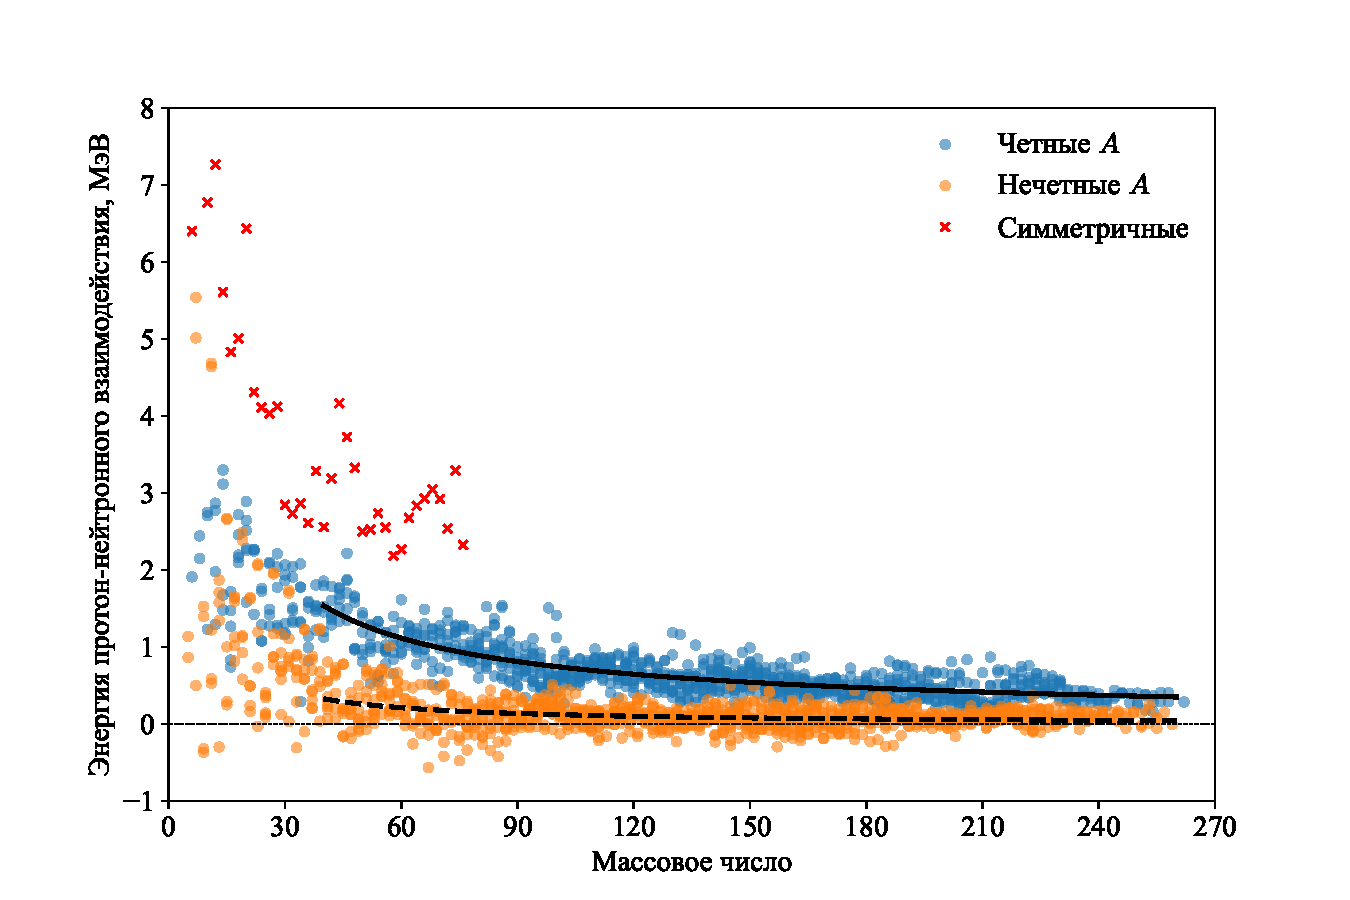
\includegraphics[width=0.9\textwidth]{../pics/delta_np.pdf}
  \caption{Экспериментальная зависимость величины $\Delta_{np}$ от массового числа, построенная по данным AME2020~\cite{huang2021}. Разными цветами отмечены четные и нечетные ядра, а также ядра с равным числом протонов и нейтронов. Черными линиями показаны аппроксимации зависимости, полученные в работе~\cite{vladimirova2022}.}
  \label{fig:delta_np}
\end{figure}

В ранних работах~\cite{vladimirova2021-1,vladimirova2021-2} авторы LMR2021 разбивали массив данных на несколько областей по значению массового числа, для каждого из которых делалась отдельная аппроксимация. В качестве модельной функции использовалось выражение
\begin{equation}
\Delta^\text{аппр}_{np} = C_1 + C_2 A^{-1},
\label{eq:old_approx}
\end{equation}
где $C_1$ и $C_2$ являются параметрами аппроксимации, причем для нечетных ядер полагалось $C_2 = 0$, то энергия протон-нейтронного взаимодействия, независящая от $A$. В более новой работе~\cite{vladimirova2022} была выбрана другая модельная функция:
\begin{equation}
\Delta^\text{аппр}_{np} = \alpha A^{\beta},
\label{eq:new_approx}
\end{equation}
где $\alpha$ и $\beta$ являются параметрами аппроксимации. Использование степени $\beta$ массового числа $A$ в качестве подгоночного параметра позволило отказаться от разбиения выборки исходных данных на диапазоны по массе изотопов. При этом, как показано в~\cite{vladimirova2022}, новая модельная функция~(\ref{eq:new_approx}) выигрывает у старой~(\ref{eq:old_approx}) в точности аппроксимации при использовании одной и той же исходной выборки данных.

В настоящей работе под массовой таблицей LMR2021 имеются в виду результаты работы~\cite{vladimirova2022}, в которой в качестве исходной выборки для аппроксимации использовалась последняя редакция базы данных AME2020~\cite{huang2021}. На рис.~\ref{fig:delta_np} черными линиями показаны результаты этой аппроксимации.

